\clearpage
\chapter{IMPLEMENTATION}

\section{Overview}
The implementation process for integrating Moodle with the Namaste BHU application involves several key steps, including Moodle deployment, configuration of Moodle web server and mobile applications, installation of essential plugins, and seamless integration using Namaste BHU as a proxy. This overview outlines the main components and processes involved in the implementation that will be discussed in detail later.

The implementation begins with the deployment of Moodle, the open-source learning management system, on dedicated servers or cloud-based infrastructure. Moodle is installed and configured to provide a secure and reliable platform for hosting courses, managing users, and delivering educational content.

Several essential plugins are installed and configured within Moodle to enhance its functionality and integration capabilities.

The Namaste BHU application serves as a proxy for seamless integration between Namaste BHU and Moodle, enabling one-click login or single sign-on (SSO) functionality for users. Users can access Moodle content and functionalities directly from the Namaste BHU application without the need for separate authentication, streamlining the user experience and promoting engagement with the integrated platform.

\section{Moodle Deployment}
The deployment and configuration of Moodle on an Azure instance, along with the setup of the Moodle web server and mobile application, lay the groundwork for integrating Moodle with the Namaste BHU application.

Steps involved in Moodle Deployment on an instance:
\begin{enumerate}
    \item Create a new virtual machine (VM) instance on Azure
    \item Configure the VM with the necessary resources (CPU, memory, storage) and firewall rules (http 80 \& https 443).
    \item Install and configure the Apache web server, PHP, and MySQL database on the VM.
    \item Download the latest version of Moodle from the \href{https://moodle.org}{official website}.
    \item Extract the Moodle package into the web server directory.
    \item Configure the Moodle installation by providing database connection details, site settings, and administrator credentials.
    \item Run the Moodle installation script to complete the setup process.
    \item Verify that Moodle is accessible through the VM's public IP address or domain name.
    \item Configure a cron job to automate tasks such as scheduled tasks, background processing, and data maintenance within Moodle.
\end{enumerate}

\subsection{Web Server}
Moodle web server is the component responsible for hosting and serving Moodle's web-based interface to users. It provides access to courses, resources, activities, and communication tools within the Moodle environment.

\subsubsection*{Configuration}

\textbf{Appearence}\\
Customize the appearance of Moodle to align with the branding and identity of Namaste BHU. Modify themes, colors, logos, and fonts to create a cohesive user experience.

\begin{figure}[H]
    \centering
    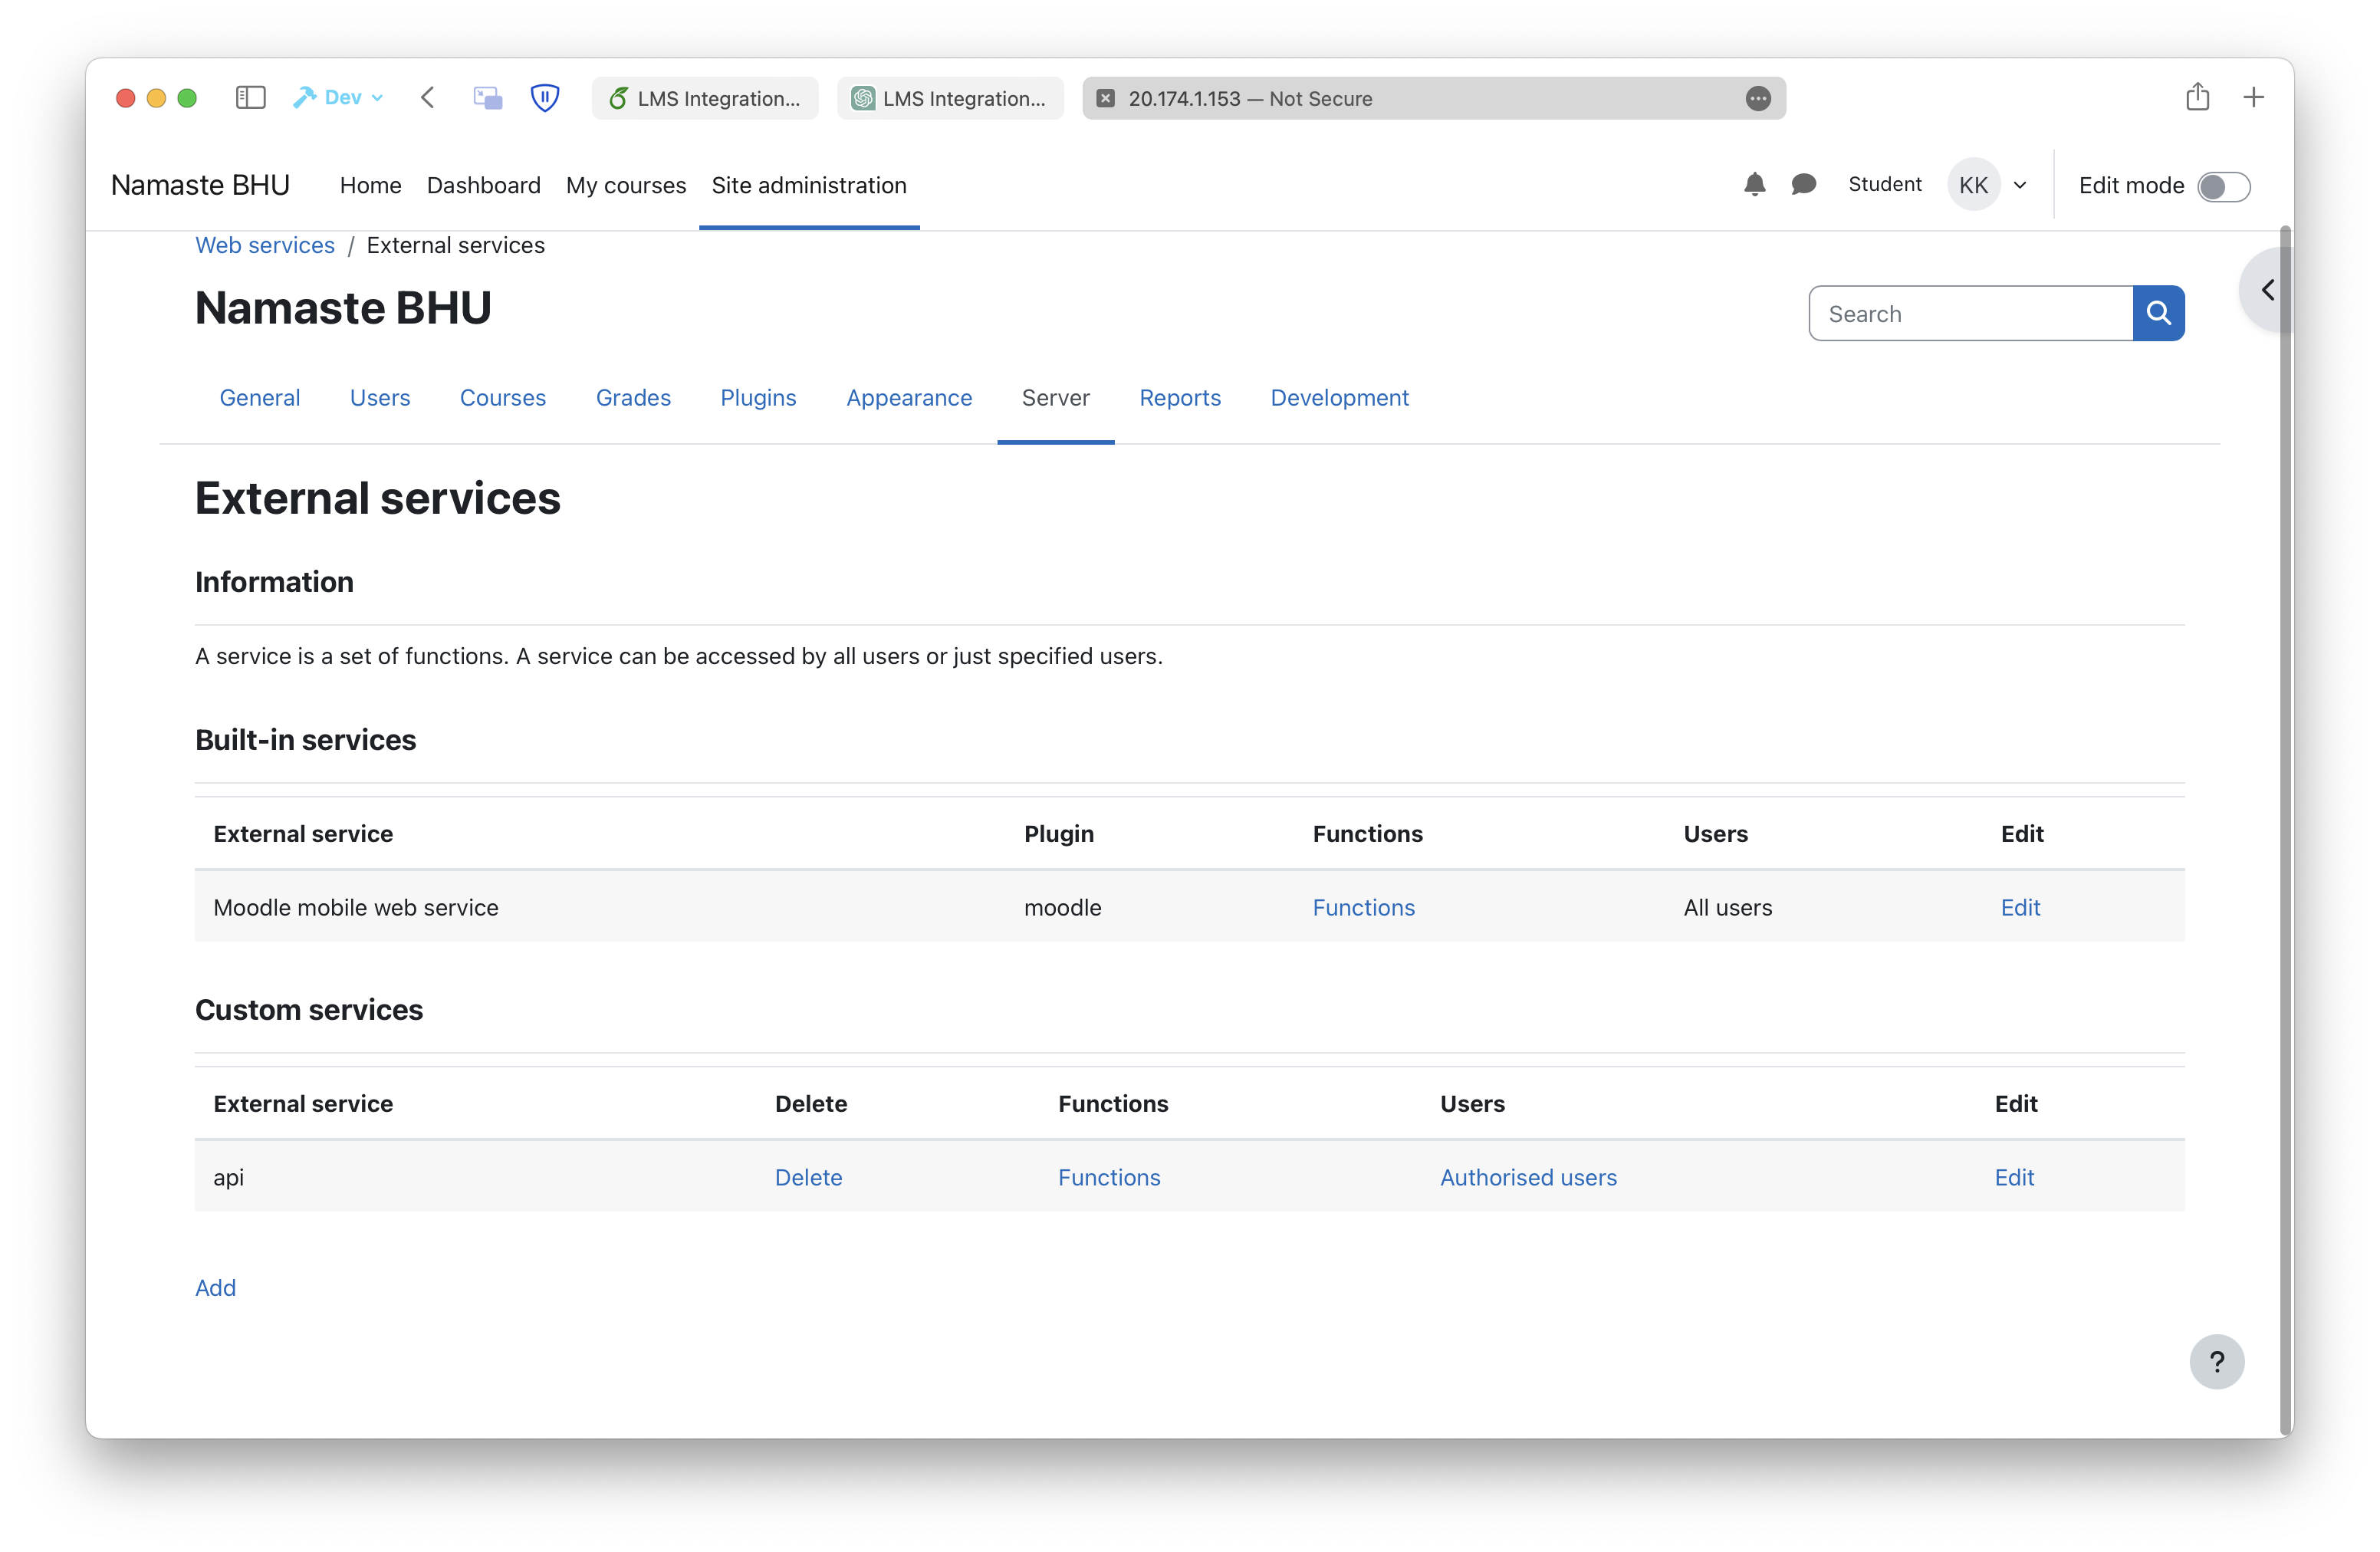
\includegraphics[width=0.75\linewidth]{assets/img/external-services.png}
    \caption{External Services}
    \label{fig:external-services}
\end{figure}

\textbf{Web Services}\\
Enable and configure web services to facilitate communication between Moodle and external systems, including Namaste BHU as show in Figure \ref{fig:external-services}. Define API endpoints, access permissions and the functionality to allow integration with external applications such as Namaste BHU.

\textbf{User Registration \& Login}\\
User registration options are configured to allow users to register manually or self-register for Moodle accounts, providing flexibility and convenience in onboarding new users and managing user accounts within the platform. Enabling login methods to provide users with options for authentication such as Manual Login and SSO from Namaste BHU.

\begin{figure}[h]
    \centering
    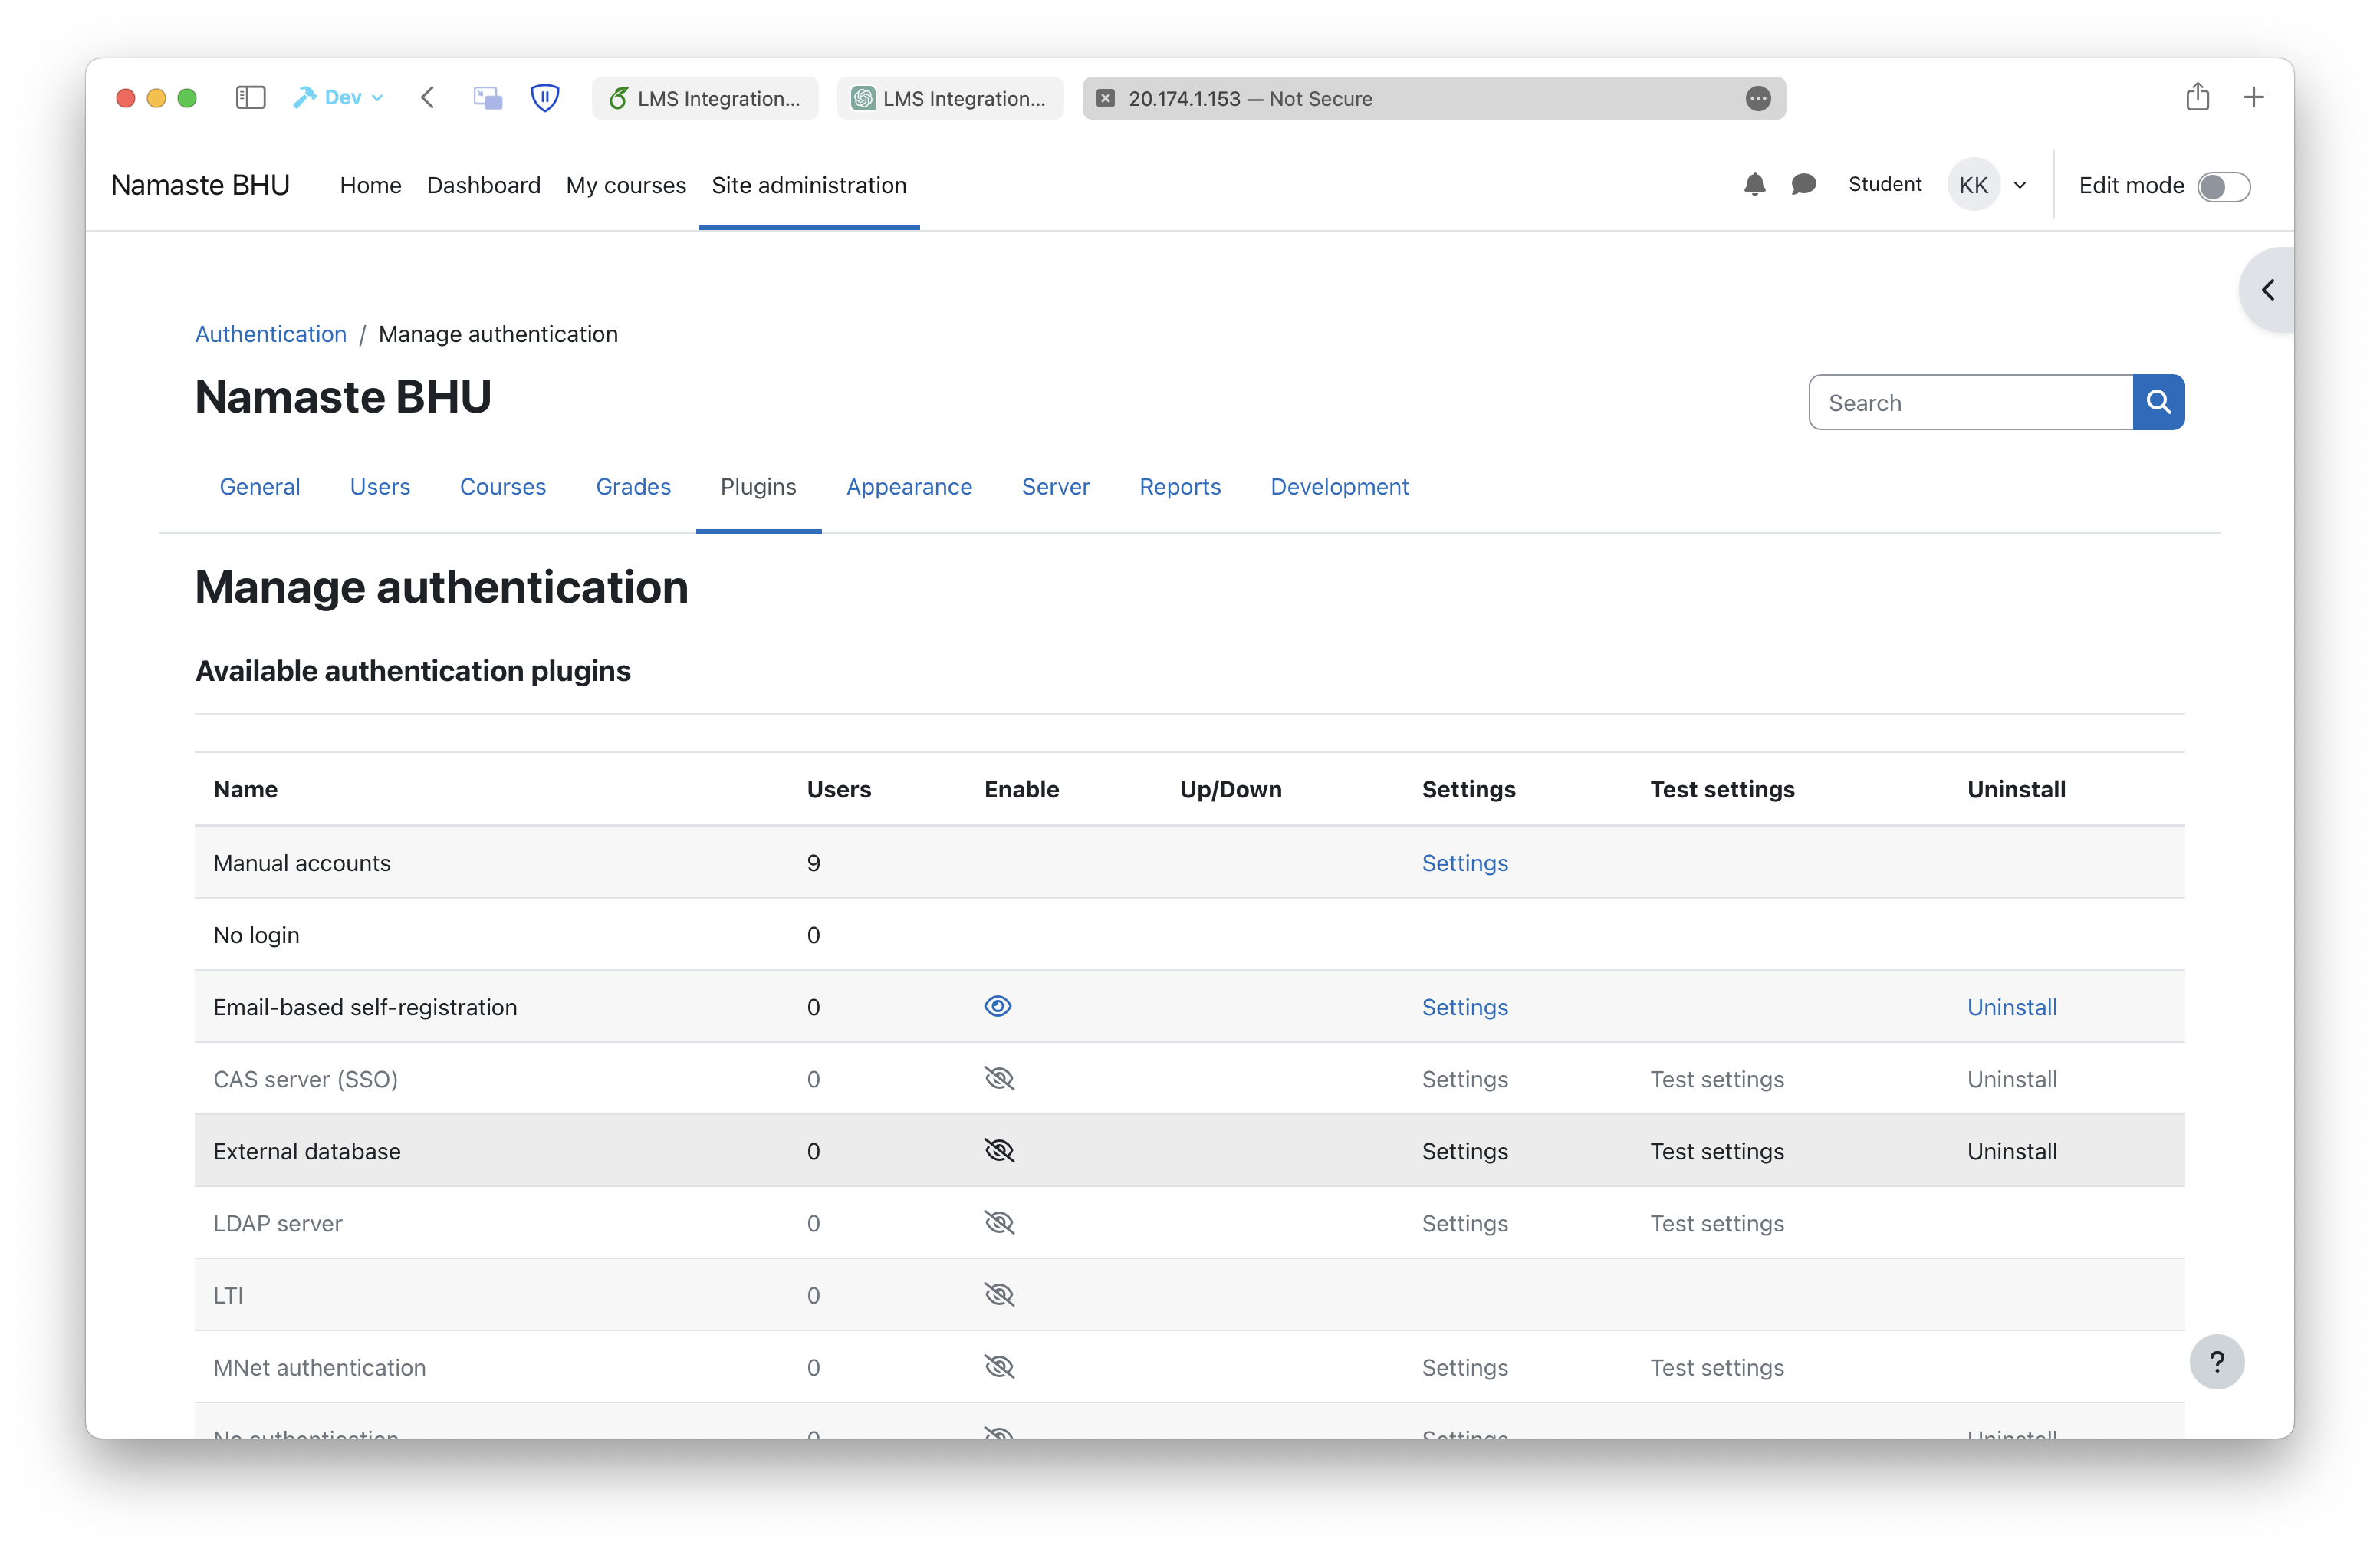
\includegraphics[width=0.75\linewidth]{assets/img/auth.png}
    \caption{Authentication}
    \label{fig:auth}
\end{figure}

\subsubsection*{Interface}

\textbf{Courses}\\
Moodle's course interface provides a centralized hub for accessing course materials, activities, resources, and communication tools, organized into categories and sections based on academic departments, programs, or topics.

\begin{figure}[H]
    \centering
    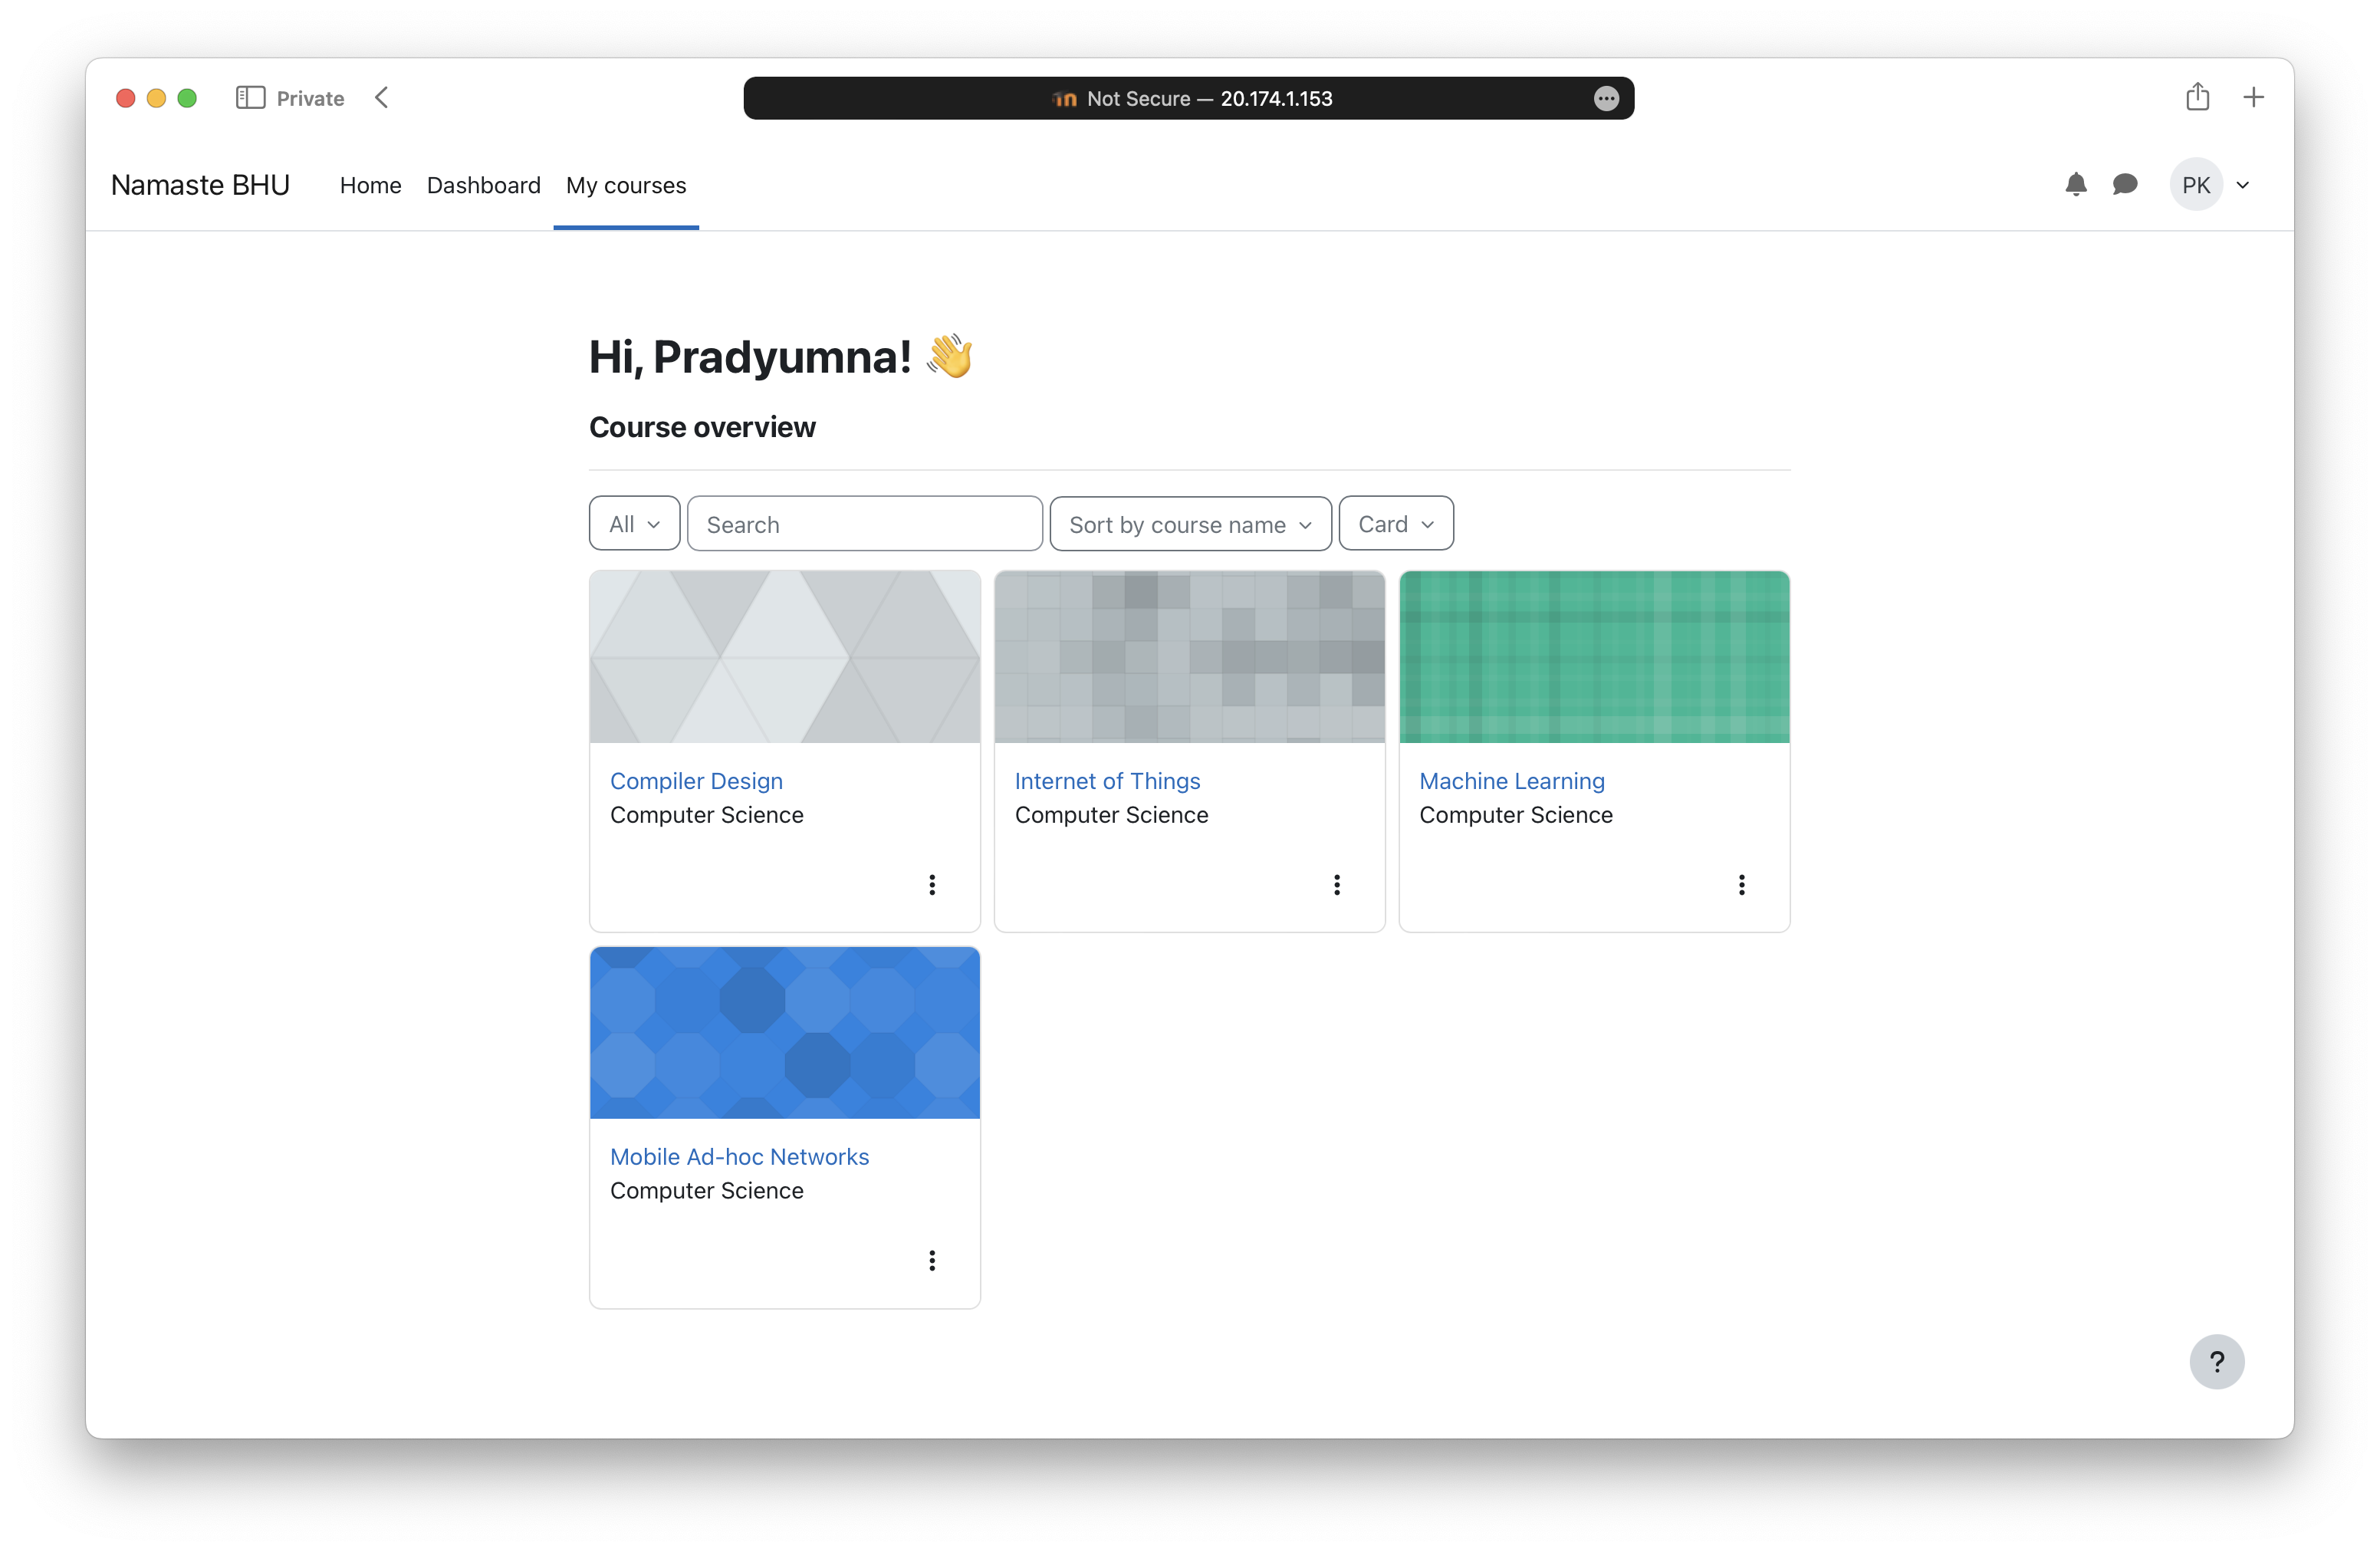
\includegraphics[width=0.75\linewidth]{assets/img/courses.png}
    \caption{Courses}
    \label{fig:courses}
\end{figure}

\textbf{Profile}\\
Users' profiles contain personalized information, preferences, and activity logs, allowing users to manage their accounts, view course enrollments, track progress, and communicate with instructors and peers.

\begin{figure}[h]
    \centering
    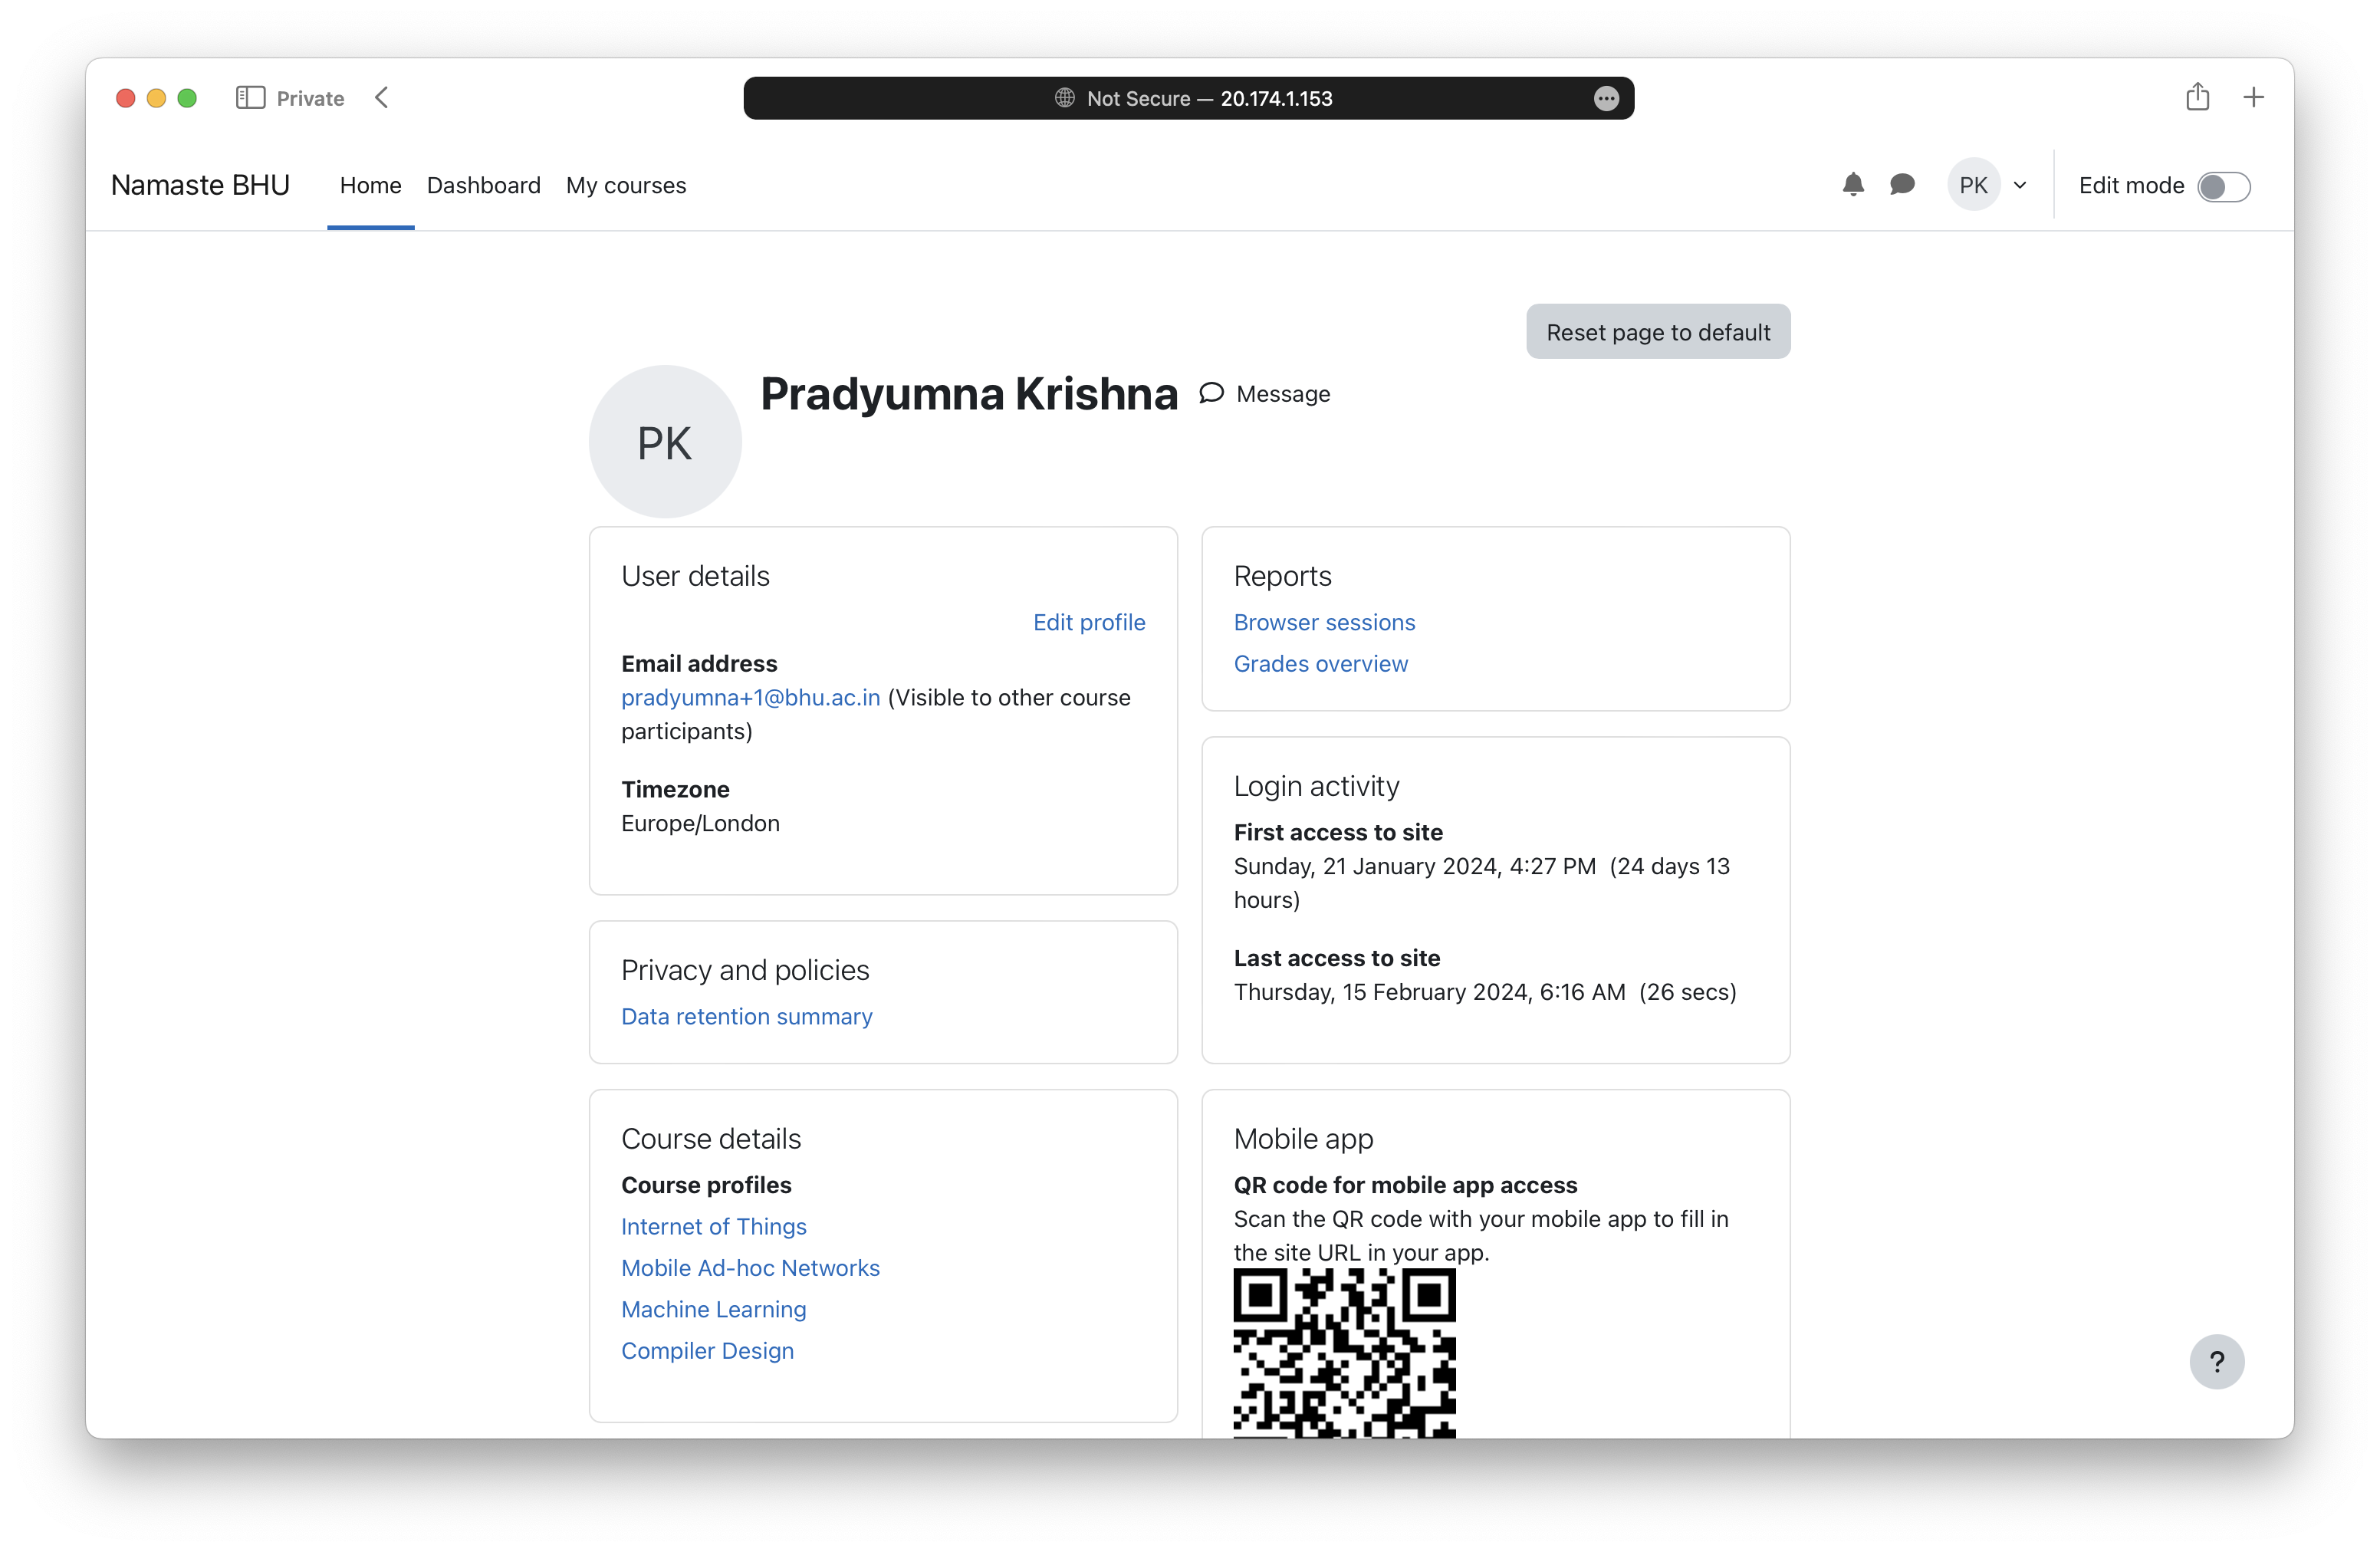
\includegraphics[width=0.75\linewidth]{assets/img/profile.png}
    \caption{Profile}
    \label{fig:profile}
\end{figure}

\subsection{Moodle Mobile}

Moodle Mobile extends the functionality of Moodle to mobile devices, providing users with access to course materials, activities, and communication tools on the go. Here's how the mobile application is enabled and configured:

\textbf{Enabling Mobile Application}\\
Enable the mobile app service in Moodle's administration settings to allow users to access Moodle through the mobile application. Configure mobile app settings, including site name, site URL, and authentication methods, to ensure compatibility and security.

\textbf{Logging through Mobile Application}\\
Users can log in to Moodle through the mobile application using their credentials from Namaste BHU or Moodle. Configure authentication settings to support seamless login and authentication, leveraging single sign-on (SSO) functionality if available.

\begin{figure}[h]
    \centering
    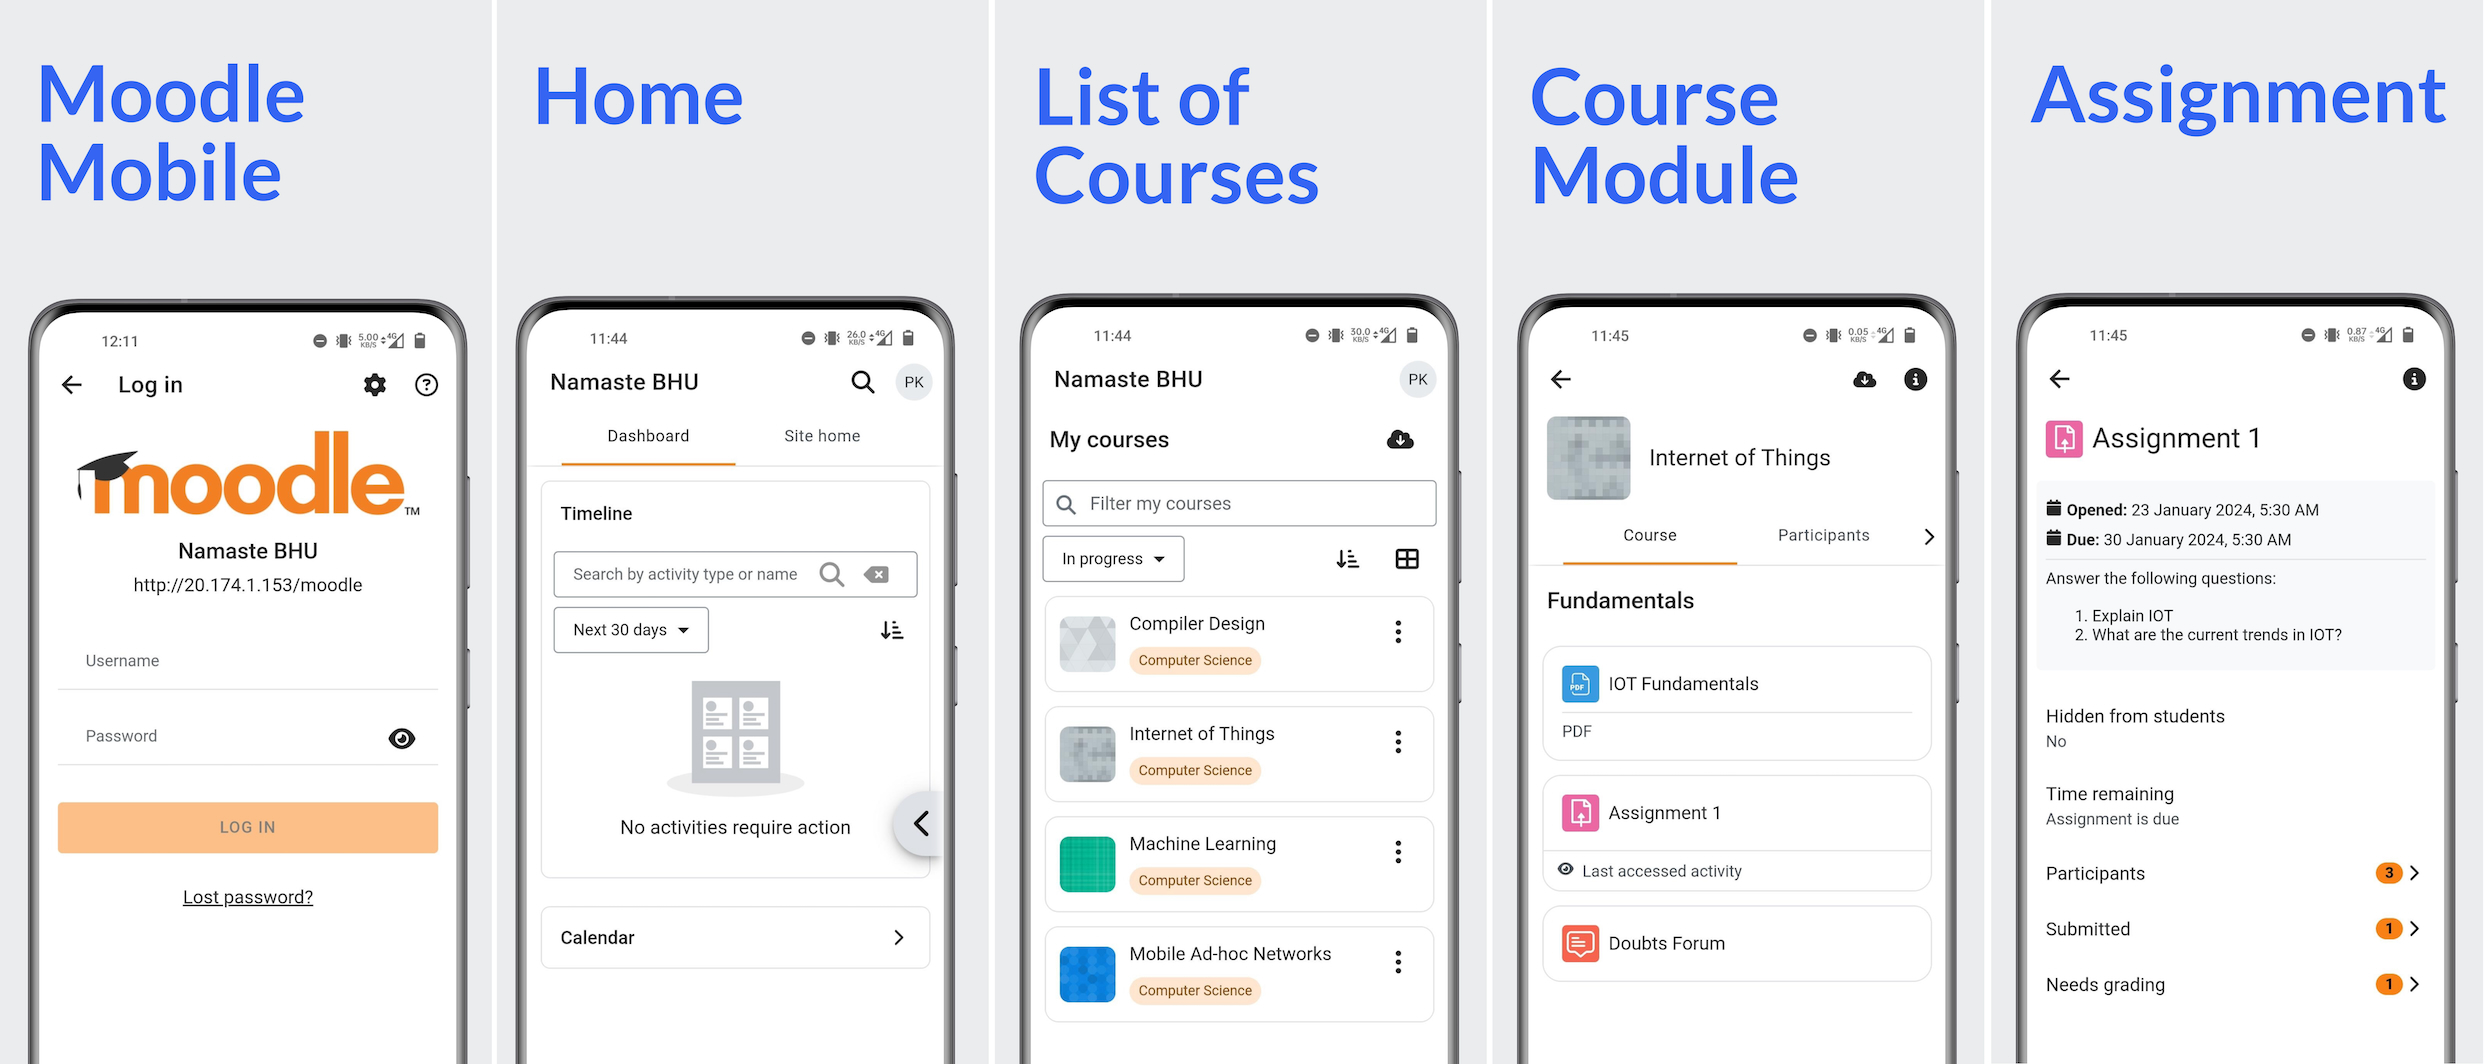
\includegraphics[width=\linewidth]{assets/img/moodle-mobile-opt.jpg}
    \caption{Moodle Mobile}
    \label{fig:moodle-mobile}
\end{figure}

\textbf{Interface and Navigation}\\
The Moodle Mobile application provides an intuitive interface and navigation experience for users, with features such as course listings, activity streams, notifications, messaging, and calendar integration. Users can easily navigate between courses, view course materials, participate in activities, and communicate with instructors and peers. The Moodle mobile interface is shown in Figure \ref{fig:moodle-mobile}.

\section{Plugins \& Extension}
These plugins and extensions enhance the functionality and capabilities of Moodle, enabling seamless integration with external systems, enhancing user experience, and extending the platform's capabilities.

\subsection{RESTful Protocol}

The \href{https://github.com/catalyst/moodle-webservice_restful}{RESTful Protocol} plugin was developed to address two main reasons: solving technical problems related to interfacing Moodle with services requiring unique URLs for each Moodle webservice call, and advancing the maturity of Moodle's webservice interface. Here are the key features of the RESTful Protocol plugin:

\begin{itemize}
    \item \textbf{Webservice Function as URL (Slash Parameter):} Instead of being passed as a query parameter, webservice functions are included in the URL. This allows each webservice to have a unique URL endpoint, enhancing accessibility and manageability.
    \item \textbf{Webservice Authorization Token as HTTP Header:} Authorisation tokens are passed using the 'Authorization' HTTP Header, ensuring secure communication between Moodle and external services.
    \item \textbf{Moodle Response Format as HTTP Header:} The desired Moodle response format is passed using the 'Accept' HTTP Header, providing flexibility in specifying the format of the response data.
\end{itemize}


A sample API call to fetch courses using RESTful Protocol:
\begin{minted}[breaklines=true]{http}
POST /moodle/webservice/restful/server.php/core_course_get_courses HTTP/1.1
Host: localhost
Authorization: <token>
Content-Type: application/json
Accept: application/json
[
    { 
        "id": "2",
        "shortname": "IOT",
    }
]
\end{minted}

\subsection{Auth UserKey}
The \href{https://moodle.org/plugins/auth_userkey}{Auth UserKey} plugin facilitates simple one-way Single Sign-On (SSO) between Moodle and external web applications. It allows users to log in to Moodle without typing their username and password by generating one-time login URLs. Here are the main features of the Auth Userkey plugin:

\begin{itemize}
    \item \textbf{Web Call to Moodle}: External applications make a web call to Moodle and provide a matching field to find the required user and generate a one-time login URL.
    \item \textbf{Simple Integration}: The plugin simplifies the integration process between Moodle and external web applications, enhancing user experience and streamlining the authentication process.
\end{itemize}

This enables an endpoint for user login:
\begin{minted}[breaklines=true]{http}
GET /auth/userkey/login.php?key={token} HTTP/1.1
HOST: localhost
\end{minted}

\subsection{Airnotifier}
\href{https://github.com/dcai/airnotifier}{AirNotifier} is a user-friendly and powerful application server for sending real-time notifications to mobile and desktop applications. It provides a unified web service interface to deliver messages to multiple devices using multiple protocols.

\section{Seamless Integration}
\subsection{Flow}

The basic workflow of the integration between Moodle and Namaste BHU involves the following steps:

\begin{figure}
    \centering
    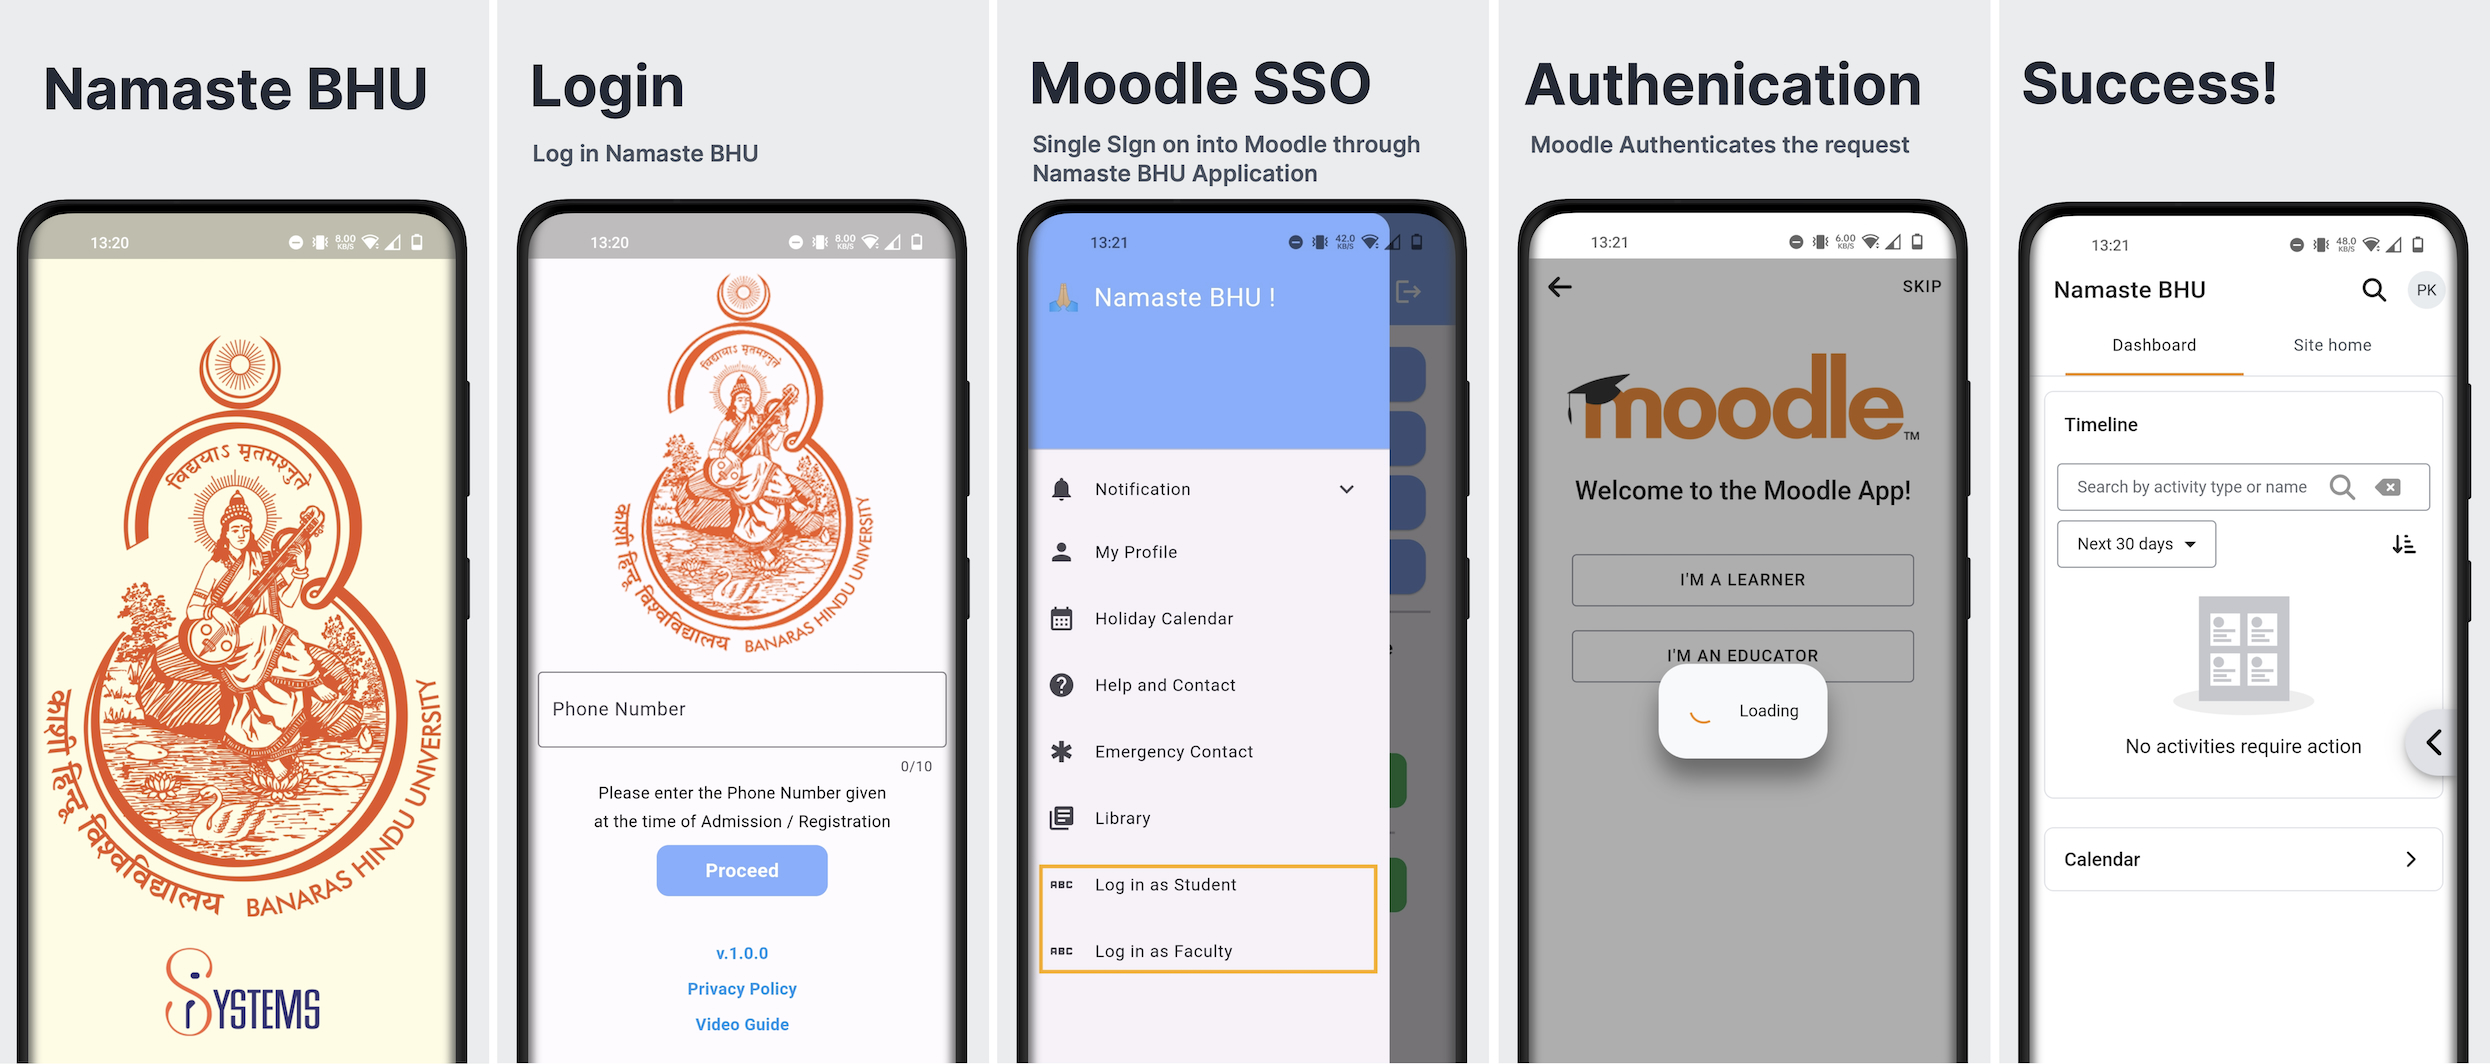
\includegraphics[width=\linewidth]{assets/img/flow-opt.jpg}
    \caption{Integration Flow}
    \label{fig:flow}
\end{figure}

\begin{enumerate}
    \item Users log in to the Namaste BHU application using their credentials.
    \item Upon successful authentication, Namaste BHU retrieves the list of courses associated with the user from its database.
    \item Namaste BHU prepares a redirection URL that includes the necessary parameters, such as the user ID, user token, redirect, and course ID.
    \item The user is redirected from Namaste BHU to Moodle through Deep Linking.
    \item Users are authenticated automatically within Moodle through token, eliminating the need for separate authentication.
    \item Upon redirection, the Moodle Mobile application accesses the course content and resources associated with the user's enrolled courses, providing seamless access to educational materials and activities.
\end{enumerate}

\subsection{Database Mapping}

Changes are required in the Namaste BHU database to facilitate seamless integration with Moodle. These changes include:

\begin{itemize}
    \item \textbf{UserID}: Namaste BHU database must store the Moodle user ID to establish a mapping between Namaste BHU users and Moodle users.
    \item \textbf{User Token}: A user token is generated and stored in the Namaste BHU database for authentication and authorization purposes when accessing Moodle resources.
    \item \textbf{Course ID}: Namaste BHU database must store the Moodle course ID to identify the courses in which users are enrolled.
\end{itemize}

These database mappings enable efficient data exchange and synchronization between Namaste BHU and Moodle, ensuring a seamless user experience.\\

\subsection{Deep Linking}
Deep linking enables users to navigate to a specific piece of content or perform a specific action within a mobile application, bypassing the app's home screen and providing a seamless user experience. It involves associating a URL with a particular location or function within the app, allowing users to access that content directly from an external source, such as a website, email, or another app.

\begin{figure}[h]
    \centering
    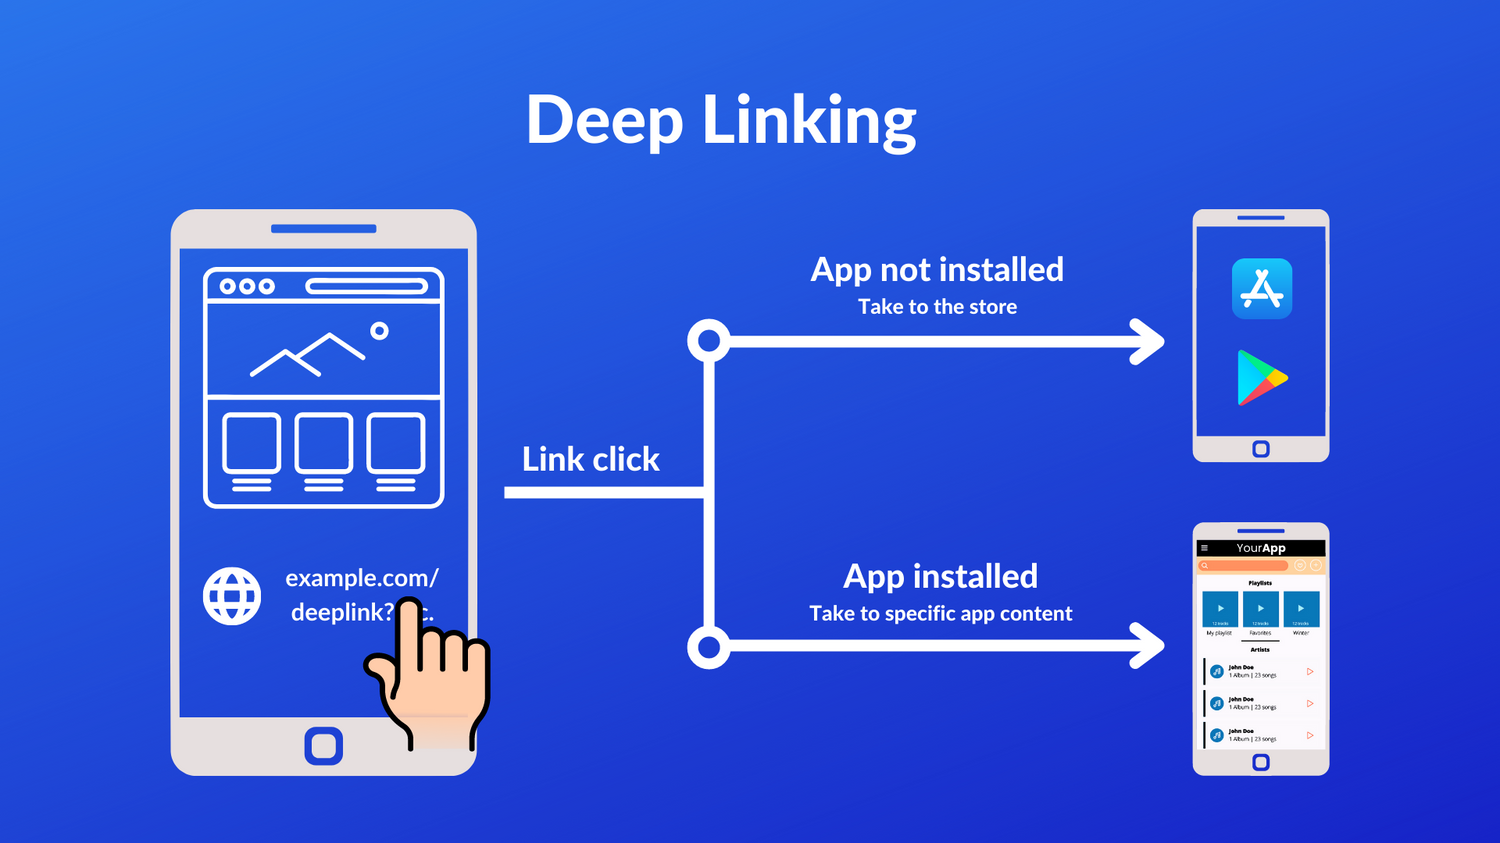
\includegraphics[width=0.75\linewidth]{assets/img/deeplinking.png}
    \caption{Deep Linking}
    \label{fig:deep-linking}
\end{figure}

\textbf{How Deep Linking Works}
\begin{itemize}
    \item Deep links typically have a specific URL structure that includes a scheme (e.g., "\texttt{https://}" or "\texttt{myapp://}"). Here, \texttt{moodlemobile://}.
    \item Mobile applications register deep links with the operating system to handle incoming link requests. This involves specifying the URL scheme and associated actions or destinations within the app.
    \item As shown in Figure \ref{fig:deep-linking} when a user clicks on a deep link, the operating system checks if the corresponding app (Moodle Mobile) is installed on the device. If the app is installed and registered to handle the deep link, the operating system opens the app and passes the link to it.
    \item The app receives the deep link and navigates the user to the specified location or performs the specified action within the app. This could involve displaying a specific screen, loading particular content, or executing a particular function.
\end{itemize}

The format to create the links for Moodle Mobile is the following:
\begin{minted}[breaklines=true]{text}
    moodlemobile://https://username@domain.com?token=TOKEN &redirect=http://domain.com/course/view.php?id=2
\end{minted}



\subsection{Messaging}
The Moodle Messaging workflow involves the generation of notifications within Moodle, communication with the AirNotifier service to deliver push notifications via Firebase Cloud Messaging, and user interaction with the notifications on their devices. This seamless process ensures timely delivery of important updates, announcements, and events to users within the Moodle and Namaste BHU ecosystems, enhancing communication and engagement within the academic community.

\begin{figure}
    \centering
    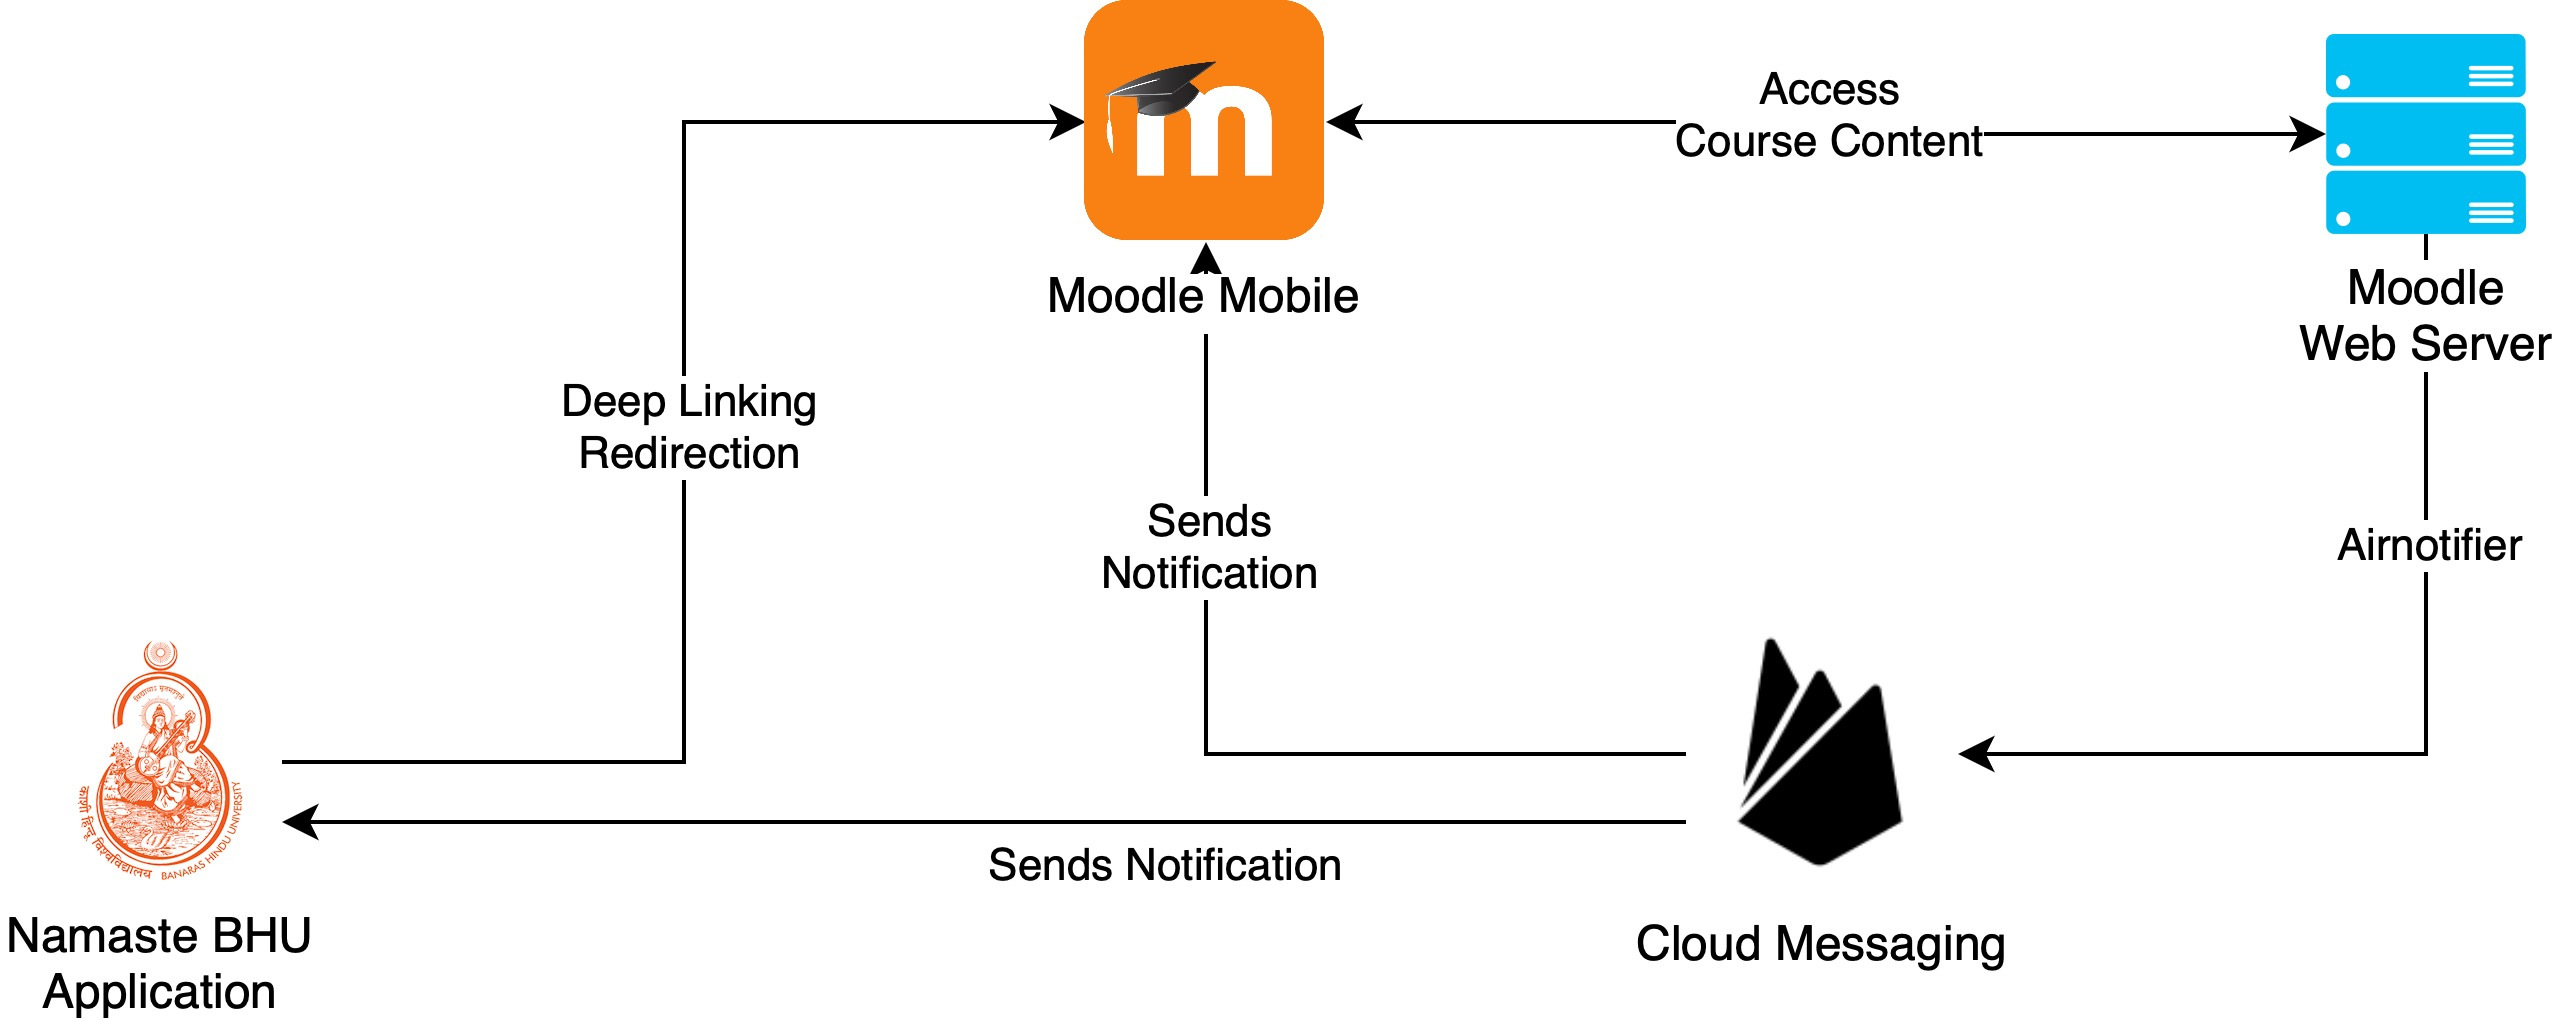
\includegraphics[width=0.75\linewidth]{assets/img/notification-flow.jpg}
    \caption{Notification Flow}
    \label{fig:notification-flow}
\end{figure}

\textbf{Workflow}\\
The Moodle platform detects a trigger event that warrants a notification, such as a new announcement, a course update, or an upcoming deadline.  Upon detecting the trigger event, Moodle generates a notification message containing relevant information, such as the event type, title, description, and associated course or user.

Moodle communicates with the AirNotifier service through its API, passing along the notification message and the device ID of the recipient. The device ID uniquely identifies the user's device and allows AirNotifier to deliver the notification to the correct recipient. 

AirNotifier utilizes Firebase Cloud Messaging (FCM) credentials to send push notifications to both Namaste BHU and Moodle Mobile applications. These credentials include the Firebase server key and project ID, which authenticate the sender and authorize the delivery of notifications through the FCM service.

Using the Firebase credentials, AirNotifier sends push notifications to the respective devices associated with the device ID provided by Moodle. The notification is delivered to the user's device through the FCM service, ensuring real-time delivery and visibility to the recipient.


\subsection{API Services}
API services are utilized for various purposes to manage both Namaste and Moodle servers, including:

\begin{itemize}
    \item \textbf{Course Management}: Creating, updating, and managing courses within Moodle through API calls from the Namaste BHU application.
    \item \textbf{User Management}: Creating, updating, and managing user accounts within Moodle through API calls from the Namaste BHU application.
    \item \textbf{Authentication}: Authenticating users and generating access tokens for accessing Moodle content through API calls from the Namaste BHU application.
    \item \textbf{Data Synchronization}: Synchronizing user data, course information, and other relevant data between Namaste BHU and Moodle databases through API services to ensure consistency and accuracy.
\end{itemize}
